\chapter{Lower bounds for homogeneous depth four circuits}\label{chap:d4hom}

The model for which we shall be interested in proving lower bounds are homogenous depth four circuits. 
These circuits compute polynomials of the form
\[
f \spaced{=} \sum_{i} Q_{i1}\dots Q_{ia_i}
\]
where each $Q_{ij}$ is a homogeneous polynomial. 
This immediately forces that $\sum_{j=1}^{a_i} \deg(Q_{ij}) = \deg(f)$ for all $i$. \\

{\bf Goal. } Find an explicit polynomial $f$ (of degree $d$, and over $n$ variables) such that any homogeneous depth four circuit requires size $n^{\Omega(\sqrt{d})}$. 
That is, if
\[
f \spaced{=} \sum_{i} Q_{i1}\dots Q_{ia_i}
\]
for homogeneous polynomials $Q_{ij}$'s, then the total number of monomials present among the $Q_{ij}$'s must be $n^{\Omega(\sqrt{d})}$. 

\subsection*{Intuition towards the measure - (1)}

Consider an expression of the form
\[
C \spaced{=} \sum_{i=1}^s Q_{i1}\dots Q_{ia_i}
\]
We shall call a summand $Q_{i1}\dots Q_{ia_i}$ \emph{good} if the degree of each $Q_{ij} \leq \sqrt{d}$. 
Let us split the above sum into \emph{good} terms and the rest. 
\begin{eqnarray}
C_1 &=& \sum_{i=1}^{s_1} Q_{i1}\dots Q_{ia_i} \spaced{\text{where}} \deg(Q_{ij}) \leq \sqrt{d} \spaced{\text{for all $i,j$}}\label{eqn:int11}\\
C_2 &=& \sum_{i=s_1+1}^{s} Q_{i1}\dots Q_{ia_i} \spaced{\text{where}} \deg(Q_{i1}) > \sqrt{d} \spaced{\text{for all $i > s_1$}}\label{eqn:int12}
\end{eqnarray}

If one were to just prove a lower bound for (\ref{eqn:int11}), then using the dimension of shifted partial derivatives we can obtain a lower bound of $n^{\Omega(\sqrt{d})}$. 
Hence let us focus on an expression of the form (\ref{eqn:int12}) and see if we can come up with a measure that gives a $n^{\Omega(\sqrt{d})}$ lower bound there as well. 

Starting with (2), let us expand each $Q_{i1}$ as a sum of monomials to obtain an expression of the form
\[
C_2 \spaced{=} \sum_{i=1}^{s'} m_i\cdot  Q_i'
\]
where each $m_i$ is a monomial of degree greater than $\sqrt{d}$, and $Q_i'$ some polynomial of degree $d - \deg(m_i)$. 
The number of summands $s'$ would be at most the size of the circuit we started out with.\\

{\bf Key Idea:} Suppose the polynomial $C_2$ was multilinear, i.e. the degree in each variable is bounded by $1$. 
Further, say $s' \leq n^{\sqrt{d}/10}$. 
Apply a random restriction $\rho$ on the variables by setting each variable independently to zero with probability $p < \frac{1}{n^{1/20}}$. 

If $m$ was any monomial that was divisible by $\sqrt{d}$ disjoint variables, then $\rho(m) \neq 0$ with probability at most $\frac{1}{n^{\sqrt{d}/20}}$. 
Hence, the probability that $\rho(m_i) \neq 0$ for some $i\leq s'$ that is divisible  by $\sqrt{d}$ variables is at most $\frac{1}{n^{\sqrt{d}/10}}$. 
Hence, the only terms that would survive on the RHS are terms of the form $\rho(m_i \cdot Q_i')$ where $m_i$ is divisible by at most $\sqrt{d}$ distinct variables. 
But recall that $\deg(m_i) > \sqrt{d}$ and this implies that $m_i$ is non-multilinear. 
If that is the case, then every monomial on the RHS is non-multilinear! 
Thus as long as $\rho(C_2) \neq 0$, there would be at least one multilinear monomial that survives. 
This would contradict our original assumption that $s' \leq n^{\sqrt{d}/10}$, giving us the lower bound we were after. \\

Thus, the measure for the sum of \emph{good} terms is the dimension of shifted partial derivatives. 
The measure for the sum of non-\emph{good} terms was \emph{the number of non-zero multilinear monomials after a random restriction}. 
Hopefully some combination of these measures would give us a measure for their sum.\footnote{There are some instances when this strategy can fail spectacularly. 
See \cite{KS14a}}

\subsection*{Intuition towards the measure - (2)}

The idea of using random restrictions as defined above essentially kills all monomials that are divisible by `too many' variables. 
Let us consider an extreme case where every monomials in each $Q_{ij}$ is just a power of a single variable. 
We shall first try to prove a lower bound for expression of the form
\[
C\spaced{=} \sum_{i}Q_{i1}\cdots Q_{ia_i}
\]
where every monomial in any $Q_{ij}$ is a power of a single variable, i.e. each $Q_{ij}$ is a sum of univariate polynomials. 

Define the operator $\mathrm{MultiQuad}$ that acts on any polynomial $Q$ such that $\mathrm{MultiQuad}(Q)$ is just the sum of monomials of $Q$ of degree at most $2$ in every variable. 
Then,
\begin{eqnarray*}
C &=&  \sum_{i}\mathrm{MultiQuad}(Q_{i1})\cdots \mathrm{MultiQuad}(Q_{ia_i}) \spaced{+} \text{other terms}\\
  & = & \qquad C_1 \spaced{+} C_2
\end{eqnarray*}

Notice that $C_1$ corresponds to a $\SPSPfanin{d/2}{2}$ circuit since we assume that each $Q_{ij}$ is a sum of univariates. 
The dimension of shifted partial derivatives would yield a lower bound for such $\SPSPfanin{d/2}{2}$ circuits. 
But what really happens to $C_2$ as we take some partial derivative?\\

{\bf Key Observation. } For any multilinear monomial $m$, the partial derivative $\partial_m(C_2)$ only consists of non-multilinear monomials. \\

Thus, this points towards the following modification of the traditional dimension of shifted partial derivatives: 
\begin{quote}
  For any polynomial $P$, look at the set of polynomials of obtained as $m_1 \cdot \partial_{m_2}(P)$ where $m_1$ and $m_2$ are \emph{multilinear monomials} of a certain degree, and compute the dimension of the \emph{multilinear component} of these polynomials i.e. erase all monomials that are non-multilinear and then compute the dimension of the residual polynomials. 
\end{quote}
This basically allows us to completely ignore the contribution of $C_2$ as we have that multilinear component of $m_1 \partial_{m_2}(C_2))$ is zero for every $m_1$ and $m_2$ that are multilinear. \\


Both these point us to a modification of the shifted partials, which \cite{KLSS,KS14} refer to as \emph{projected shifted partial derivatives}. 

\begin{definition}[Projected Shifted Partial Derivatives]\label{defn:PSPD}
Fix parameters $k,\ell > 0$. 
For any polynomial $P$, the set of projected shifted partials of $P$, denoted by $\mathrm{PSD}_{k,\ell}(P)$ is defined as follows
\[
\mathrm{PSD}_{k,\ell}(P) \spaced{=} \setdef{\mathrm{mult}(m_1 \cdot \partial_{m_2}(P))}{\begin{array}{c}\deg(m_1) = \ell\;,\; \deg(m_2) = k,\\ \text{$m_1$ and $m_2$ are multilinear}\end{array}}
\]
where $\mathrm{mult}(f)$ refers to the polynomial $f$ projected to only the multilinear monomials of $f$. 

The measure $\Gamma^{\mathrm{PSD}}_{k,\ell}(P)$ is defined as the dimension of the above set of polynomials, i.e.
\[\Gamma^{\mathrm{PSD}}_{k,\ell}(P) \spaced{=} \dim\inparen{\mathrm{span}(\mathrm{PSD}_{k,\ell})}\qedhere\]
\end{definition}

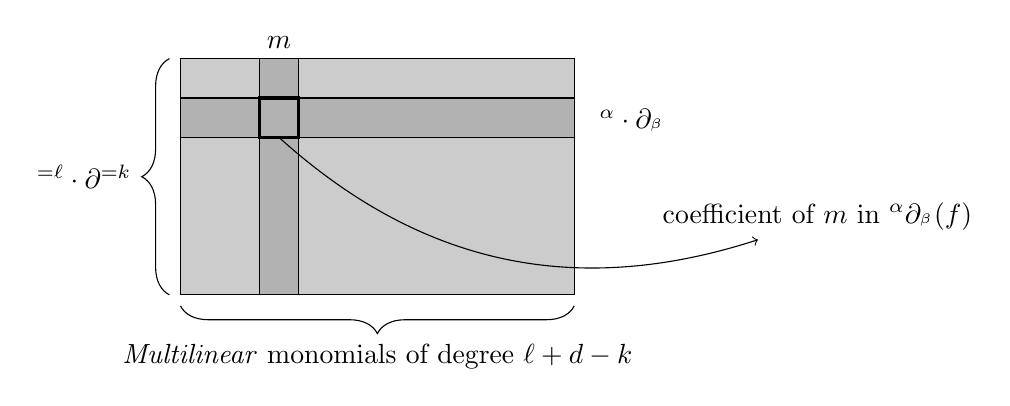
\begin{tikzpicture}
\draw[fill=black!20] (0,0) rectangle (5,3);

\draw[decorate,decoration={brace,amplitude=10pt,raise=4pt},yshift=0pt]
(0,0) -- (0,3);
\node[anchor=east] at (-0.5,1.5) {$\vecx^{=\ell} \cdot \partial^{=k}$};
\draw[decorate,decoration={brace,amplitude=10pt,mirror, raise=4pt},yshift=0pt] 
(0,0) -- (5,0);
\node[anchor=north] at (2.5,-0.5) {\emph{Multilinear} monomials of degree $\ell + d - k$};

\draw[fill=black!30] (1,0) rectangle (1.5,3);
\node at (1.25,3.2) {$m$};

\draw[fill=black!30] (0,2) rectangle (5,2.5);
\node[anchor=west] at (5.2,2.2) {$\vecx^{\alpha} \cdot \partial_{\vecx^\beta}$};

\draw[very thick] (1,2) rectangle (1.5,2.5);

\node[anchor=west] at (6,1) {coefficient of $m$ in $\vecx^\alpha \partial_{\vecx^\beta}(f)$}
edge[<-,bend left] (1.25,2);
\end{tikzpicture}


The works of \cite{KLSS,KS14} use this measure to prove a lower bound for ``\emph{low-support} depth $4$ circuits''. 
As sketched earlier, the task of proving lower bounds for general homogeneous depth $4$ circuits can be reduced to the \emph{low-support} depth $4$ circuits via random restrictions. 

\section{Reducing to `low-support' depth $4$ circuits}\label{sec:red-to-low-support}

We have already seen a sketch of how this can be done via a random restriction but let us formalize this as a lemma. 

\begin{lemma}\label{lem:red-to-low-supp}
Let $P$ be an $n$-variate degree $d$ polynomial computed by a homogeneous depth $4$ circuit $C$ of size $s \leq n^{c\sqrt{d}}$, for some $c>0$. 
Let $\rho$ be a random restriction that sets each variable to zero independently with probability $1 - 1/n^{2c}$. 
Then with probability at least $(1 - 1/s)$, the polynomial $\rho(P)$ is computed by a homogeneous depth $4$ circuit $C'$ with bottom support at most $\sqrt{d}$ and size at most $s$. 
\end{lemma}
\begin{proof}
Let $\inbrace{m_1,\dots, m_r}$ be the set of all monomials computed at the lowest layer of the depth $4$ circuit $C$ that are divisible by more than $\sqrt{d}$ distinct variables. 
Since the size of $C$ is at most $s$, we also have that $r\leq s$. 
Then,
\begin{eqnarray*}
\forall i\in [r] \qquad \Pr[\rho(m_i) \neq 0] & \leq & \frac{1}{n^{2c\sqrt{d}}}\\
\implies \qquad \Pr[\exists i \;:\; \rho(m_i) \neq 0] & \leq & \frac{r}{n^{2c\sqrt{d}}} \leq \frac{1}{n^{c\sqrt{d}}} \leq \frac{1}{s}
\end{eqnarray*}
Thus, with probability at least $(1 - 1/s)$, all the large support monomials are killed and $C$ reduces to a homogeneous depth $4$ circuit of bottom support at most $\sqrt{d}$. 
\end{proof}

\subsection{Handling random restrictions}

The previous section outlined how in essence, it would suffice to try and find an explicit polynomial for which we can prove a good enough lower bound for bounded bottom-support depth $4$ circuits. 
Let us say that we have found an explicit polynomial $g$ that requires depth $4$ circuits of size at least $n^{\sqrt{d}/100}$. 
Are we done? Let us write things down formally to see exactly what we need. 

Say the polynomial we wish to show requires large homogeneous depth $4$ circuits is $f$. 
Let us assume on the contrary that $f$ can be computed by homogeneous depth $4$ circuits of size $s < n^{\sqrt{d}/10000}$. 
Then, by \autoref{lem:red-to-low-supp}, $\rho(f)$ can be computed by a homogeneous depth $4$ circuits of bottom support bounded by $\sqrt{d}/1000$ of size $s$. 
We want to be able to say that this is a contradiction. 
We might be able to say that if $\rho(f)$ has $g$ as \emph{a projection}, that is, but setting more variables to zero in $\rho(f)$ we obtain $g$. 

Both the results of \cite{KLSS} and \cite{KS14} proceed by showing that the polynomial $g$, for which they show a lower bound for bounded bottom support circuits, is robust enough to yield the lower bound even after random restriction. 
The calculations become trickier because the calculations of $\Gamma^{[\mathrm{PSD}]}_{k,\ell}(\rho(f))$. 
However, in this survey we shall use an easier approach to generically lift any $g$ to a different polynomial $f$ such that $\rho(f)$ has $g$ as a projection. 
This trick came up during discussions with Mrinal Kumar. 

\begin{lemma}\label{lem:lin-transform-trick}
Let $\rho$ be a random restriction that sets each variable to zero independently with probability $1 - p$. 
For any polynomial $f(y_1,\dots y_n)$, define $f \circ \mathrm{Lin}_p$ as
\[
f \circ \mathrm{Lin}_p \spaced{=} f\inparen{\sum_{i=1}^t y_{1i}, \cdots, \sum_{i=1}^t y_{nt}}\quad \text{where $t = \inparen{\frac{1}{p}} n \log n$}
\]
Then, $\rho(f \circ \mathrm{Lin}_p)$ has $f$ as a projection with probability $1 - 1/2^{n}$. 
\end{lemma}
\begin{proof} For any $i = 1, \dots, n$
\begin{eqnarray*}
\quad \Pr[\rho(y_{i1}) = \dots \rho(y_{it}) = 0 ] & = & \inparen{1 - p}^t\\ 
& = & \frac{1}{n\cdot 2^n}\\
\implies \Pr[\exists i\;:\;\rho(y_{i1}) = \dots \rho(y_{it}) = 0 ]  & \leq  & \frac{1}{2^n} 
\end{eqnarray*}
Hence, with probability at least $1 - 1/2^n$, for each $i$ there is some $j$ such that $\rho(y_{ij}) \neq 0$. 
Therefore, with probability at least $1 - 1/2^n$, the polynomial $f$ is a projection of $\rho(f \circ \mathrm{Lin}_p)$. \end{proof}

In all the applications, as in \autoref{lem:red-to-low-supp}, we would have $p = 1/n^{O(1)}$. 
Thus, we would only incur a polynomial blow-up in the number of variables from $f$ to $f\circ \mathrm{Lin}_p$. 
Hence, we can focus on proving a lower bound  a homogeneous depth $4$ circuit of bottom support at most $r$ (which would eventually be something like $\sqrt{d}/100$). 

\begin{lemma}[\cite{KLSS}]\label{lem:upper-bound-low-supp}
Let $P$ be an $n$-variate degree $d$ polynomial computed by a homogeneous depth $4$ circuit of size $s$ and bottom-support at most $r$. 
Then for any $k,\ell$ such that $\ell + rk \leq n/2$, 
\[
\Gamma^{\mathrm{PSD}}_{k,\ell}(P) \quad \leq \quad s \cdot \binom{\frac{2d}{r}+k}{k}\cdot \binom{n}{\ell+rk}. 
\]
\end{lemma}

The proof of this lemma is exactly along the description in of Intuition - (2): split the circuit into multiquadratic and non-multiquadratic part, and show that the non-multiquadratic part contributes no multilinear monomials. 
But to just put things in perspective, we shall be dealing with parameters $r = \sqrt{d}/100$, $k = \sqrt{d}$ and $\ell = \frac{n}{2}(1 - \epsilon)$ for $\epsilon = O\inparen{\frac{\log d}{\sqrt{d}}}$. 
The above bound, by \autoref{lem:binom-approx}, can be seen to reduce to
\[
\Gamma^{\mathrm{PSD}}_{k,\ell}(P) \quad \leq \quad s \cdot \binom{n}{\ell} \cdot (1+\epsilon)^{2rk} \cdot 2^{O(\sqrt{d})}
\]


\subsection*{Sanity checks}

Let us first check if this measure can at least in principle yield a lower bound for us. 
The best way to do this is to get some heuristic estimate of what we expect the measure to be for a random $n$-variate degree $d$ polynomial $R$. \\

{\bf Heuristic Estimate. } For a random $n$-variate degree $d$ polynomial $R$, we expect the $\Gamma^{\mathrm{PSD}}_{k,\ell}(R)$ to be as large as it can be, i.e.
\[
\Gamma^{\mathrm{PSD}}_{k,\ell}(R) \spaced{\approx} \min\inparen{\binom{n}{k}\cdot \binom{n}{\ell}, \binom{n}{\ell + d-k}}
\]

As a first step, one should first check that if we could indeed find a polynomial $P$ for which the bound is as large as stated above, do we get a useful lower bound from \autoref{lem:upper-bound-low-supp}? Turns out that if we were to choose our parameters carefully, we do indeed get the lower bound. 
Just to give a sense of how \emph{careful} we need to be, here is some of the parameters that are chosen in \cite{KLSS,KS14}. 

\begin{itemize}
\item The number of variables $n$ is at least the cube of the degree $d$. 
\item The model we shall be working with is bottom-support $r$ where $r = \sqrt{d}/1000$. 
\item The order of derivatives $k = \sqrt{d}$. 
\item The degree of the shift $\ell$ shall be chosen as $\ell = \frac{n}{2}\inparen{1 - \epsilon}$ where $\epsilon = \frac{\log d}{c\sqrt{d}}$ for a suitable constant $c$. 
\end{itemize}

The above choice of parameters might already seem pretty fragile but these are not the most delicate choices! 
While proving the lower bound on $\Gamma^{\mathrm{PSD}}_{k,\ell}$ for an explicit polynomial, the number of monomials etc. need to be tailored to perfection to make the proof work. 

\section{The surrogate rank approach of \cite{KLSS}}

The goal is now to find an explicit polynomial $P$ such that $\mathrm{PSD}_{k,\ell}(P)$ has large rank. 
One way to prove that a set of polynomials are linearly independent is to show that they have distinct leading monomials (as used \cite{gkks13} etc.) Another method is to show that these polynomials are \emph{almost orthogonal}. 
An example of this phenomenon can be seen in the following fact. 

\begin{fact}
Let $M$ be a square matrix such that the absolute value of the diagonal entry is larger than sum of the absolute values of the non-diagonal entries in that row or column, i.e. $\abs{M_{ii}} \geq \sum_{j\neq i} \abs{M_{ij}}$ for all $i$. 
Then the matrix $M$ is full rank. 
\end{fact}

Such matrices are also called \emph{diagonally dominant matrices}, and captures the notion of \emph{almost orthogonal} vectors alluded to earlier. 
For symmetric matrices $M$, the following bound of Alon~\cite{Alo09}.

\begin{lemma}[\cite{Alo09}]\label{lem:trace-bound} For any real symmetric matrix $M$, 
\[
\rank(M) \spaced{\geq} \frac{(\mathrm{Tr}(M))^2}{\mathrm{Tr}(M^2)}
\]
\end{lemma}

We'll see the proof of this shortly but it would shed some more intuition to see what the above lemma yields for a diagonally dominant matrix. 
Let $M$ be a matrix of the form
\[
M \spaced{=} \insquare{\begin{array}{cccc}
D &  d & \dots &  d\\
 d & D & \dots & d\\
\vdots & \vdots & \ddots & \vdots \\
d & d & \dots & D
\end{array}}_{r \times r}
\]
Then, $\mathrm{Tr}(M) = D\cdot r$, and $\mathrm{Tr}(M^2) = (D^2 + (r-1)d^2)r = O(D^2 r + r^2 d^2)$. 
If $D > (r-1)d^2$, then $\mathrm{Tr}(M^2) = O(D^2r)$. 
Thus, the above lemma gives that $\rank(M) = \Omega(r)$. 
\begin{proof}
By the spectral theorem, any real symmetric matrix has a basis of eigen vectors with eigenvalues $\lambda_1,\dots, \lambda_n$ where $n$ is the dimension of the matrix. 
If $\lambda_1,\dots, \lambda_r$ are the non-zero eigenvalues, then 
\begin{eqnarray*}
\mathrm{Tr}(M) &   =  & \sum_{i=1}^r \lambda_i\\
& \leq & \sqrt{r} \;\cdot \; \inparen{\sum_{i=1}^r \lambda_i^2} = \sqrt{r}\;\cdot \; \mathrm{Tr}(M^2)\\
\implies r & \geq & \frac{(\mathrm{Tr}(M))^2}{\mathrm{Tr}(M^2)}
\end{eqnarray*}
\end{proof}

The bound of \cite{KLSS} for an explicit polynomial $P$ proceeds by considering the matrix $B$ where each row is indexed by a pair of multilinear monomials $(m_1,m_2)$  of degree $k$ and $\ell$ respectively, and the row is just the coefficients of the monomials of $\mathrm{mult}(m_2 \partial_{m_1}(P))$ in a fixed order. 
Note that $B$ is not even a square matrix, and certainly not symmetric. 
However, the matrix $M = B B^T$ is a symmetric square matrix such that $\rank(M) \leq \rank(B)$. \\

Let us spend some time understand the entries of $M$. 
The $(i,j)$-th entry of $M$ is precisely the inner-product of row $i$ and row $j$ of $B$. 
If $P$ is a polynomial with just zero-one coefficients, then the $i$-th diagonal entry is precisely the number of non-zero entries in row $i$ of $B$. 
Thus,
\begin{eqnarray*}
\mathrm{Tr}(M) & = & \text{number of non-zero entries in $B$}\\
  & = & \text{(\# cols of $B$)} \cdot \mathop{\mathbb{E}}_i[\text{\# non-zero entries in $i$-th col of $B$}] 
\end{eqnarray*}
The calculation for $\mathrm{Tr}(M^2)$ requires a little more care. 
Let $M_i$ refer to the $i$-th row of $M$ and $B_i$ refer to the $i$-th row of $B$. 
Then,
\begin{eqnarray*}
\mathrm{Tr}(M^2) & = & \sum_{i} \inangle{M_i, M_i}\\
 & = & \sum_{i} \sum_j \inangle{B_i, B_j}^2 \spaced{=}\sum_{i} \sum_j \inparen{\sum_m B_{im} B_{jm}}^2\\
 & = & \sum_{i} \sum_j \sum_m B_{im}^2 B_{jm}^2  \spaced{+} \sum_i \sum_j \sum_{m\neq m'} B_{im}B_{im'}B_{jm}B_{jm'}\\
 & = & \sum_{m} \inparen{\sum_i \sum_j B_{im} B_{jm}}  \spaced{+} \sum_i \sum_j \sum_{m\neq m'} B_{im}B_{im'}B_{jm}B_{jm'}\\
 & = & \quad\quad\quad T_1 \quad\quad\quad\quad\quad\quad + \quad\quad\quad\quad\quad\quad T_2
\end{eqnarray*}
The first term $T_1$ is easy to calculate:
\begin{eqnarray*}
T_1 & = & \text{(\# cols of $B$)} \cdot \mathop{\mathbb{E}}_i[\inparen{\text{\# non-zero entries in $i$-th col of $B$}}^2] \\
 & \stackrel{\tiny \text{(hopefully)}}{\approx} & \text{(\# cols of $B$)} \cdot \mathop{\mathbb{E}}_i[\inparen{\text{\# non-zero entries in $i$-th col of $B$}}]^2
\end{eqnarray*}
The term $T_2$ roughly corresponds to the number of $2\times 2$ submatrices of $B$ that is $\insquare{\begin{array}{cc}1 & 1 \\ 1 & 1\end{array}}$. 
If we could somehow show that there are not too many such submatrices, then $\mathrm{Tr}(M^2)$ is essentially dominated by $T_1$. 
That would then yield that $\rank(M) \gtrapprox \text{(\# cols of $B$)}$. 

\subsection*{Obtaining a bound on $T_2$:}

\[
T_2 \spaced{=} \sum_i \sum_j \sum_{m\neq m'} B_{im}B_{im'}B_{jm}B_{jm'}
\]
Each term $B_{im}B_{im'}B_{jm}B_{jm'}$ that is non-zero corresponds to a $2\times 2$ submatrix of $B$ (indexed by rows $i,j$ and columns $m,m'$) that is $\insquare{\begin{array}{cc} 1 & 1\\ 1&1
  \end{array}}$. \\

The columns of $B$ are indexed by multilinear monomials of degree $\ell + d - k$, and the rows of $B$ are indexed by a derivative and a shift. 
Let row $i$ correspond to $\mathrm{mult}(\gamma_1 \cdot \partial_{\alpha_1}(P))$ and row $j$ to $\mathrm{mult}(\gamma_1 \cdot \partial_{\alpha_1}(P))$. 
Thus, if the $2\times 2$ minor indexed by rows $i,j$ and columns $m,m'$ equals $\insquare{\begin{array}{cc} 1 & 1\\ 1&1 \end{array}}$, then there exists $\beta_1, \beta_2,\beta_3,\beta_4 \in P$ such that
\begin{eqnarray*}
m \spaced{=} \frac{\beta_1}{\alpha_1}\cdot \gamma_1 & = & \frac{\beta_3}{\alpha_2} \cdot  \gamma_2\\
m' \spaced{=} \frac{\beta_2}{\alpha_1}\cdot \gamma_1 & = & \frac{\beta_4}{\alpha_2}\cdot \gamma_2\\
\implies \frac{\beta_1}{\beta_3} & = & \frac{\beta_2}{\beta_4}
\end{eqnarray*}
Following notation used in \cite{KLSS}, we shall call $\beta_1,\beta_2,\beta_3,\beta_4$ as the \emph{label} of the $2\times 2$ minor. 
Since $m\neq m'$, we also have that $\beta_1 \neq \beta_2$. 
What we'd like to say that the only way $\beta_1/\beta_3 = \beta_2/\beta_4$ is if $\beta_3 = \beta_1$ and $\beta_2 = \beta_4$. 
This need not be true in general of course, but this is where the choice of the polynomial comes in. 

\begin{claim}
If $P$ is the $\NW_{d,d^3, e}$ polynomial for $e = \frac{d}{3}$ then any $2\times 2$ minor of $B$ (with the order of derivatives $k = o(d)$) that is $\insquare{\begin{array}{cc} 1&1\\1&1\end{array}}$ has label $\beta_1,\beta_2,\beta_3,\beta_4$ where $\beta_1 = \beta_3$ and $\beta_2 = \beta_4$, or $\beta_1 = \beta_2$ and $\beta_3 = \beta_4$. 
\end{claim}
\begin{proof}
Assume that $\beta_1 \neq \beta_3$. 
Then by \autoref{lem:NW-low-intersection} we know that they differ in at least $2d/3$ places. 
But then, $\beta_1/\beta_3 = \beta_2/\beta_4$ forces that $\beta_1$ and $\beta_3$ must agree at least $2d/3$ places forcing $\beta_1 = \beta_2$. 
\end{proof}

Thus, for the $\NW$-polynomial the number of such boxes is quite small. 
Using this, albeit with a reasonable amount of sweat, one can estimate $T_2$ to show that $T_2 = O(T_1)$. 
Thus, \cite{KLSS} obtain the following bound. 

\begin{lemma}[\cite{KLSS}]
For the polynomial $\NW_{d,d^3,e}$, for $e = \frac{d}{3}$, and $k = \sqrt{d}$ and $\ell = \frac{n}{2}\inparen{1 - \frac{\log d}{\sqrt{d}}}$ we have the bound
\[
\Gamma^{\mathrm{PSD}}_{k,\ell}(\NW_{d,d^3,e}) \spaced{\geq} \frac{1}{\poly(n,d)} \cdot \min\inparen{\binom{n}{\ell + d - k}, \binom{d}{k}^2 \cdot d^k \cdot k! \cdot \binom{n}{\ell}}
\]
\end{lemma}
Note that the first term of the $\min$ in the RHS is the number of columns of $B$, as we had heuristically estimated. 
Simplifying the RHS using \autoref{lem:binom-approx}, we get
\[
\Gamma^{\mathrm{PSD}}_{k,\ell}(\NW_{d,d^3,e}) \spaced{\geq} \frac{1}{\poly(n,d)} \cdot \binom{n}{\ell}\cdot \exp\inparen{c\cdot \epsilon (d - k)}
\]
for some constant $c > 0$. 
Since $\epsilon = \frac{\log d}{\sqrt{d}}$, we get 
\[
\Gamma^{\mathrm{PSD}}_{k,\ell}(\NW_{d,d^3,e}) \spaced{\geq} \frac{1}{\poly(n,d)} \cdot \binom{n}{\ell}\cdot \exp\inparen{c\cdot \sqrt{d}\cdot \log d}
\]
With the above bound and \autoref{lem:upper-bound-low-supp}, we get the lower bound of \cite{KLSS}. 
\begin{theorem}[\cite{KLSS}]\label{thm:KLSS-lowsupp}
Any depth $4$ homogeneous circuit of bottom support $r = \sqrt{d}/1000$ computing the polynomial $\NW_{d,d^3,d/3}$ over a characteristic zero field must have top fan-in $s = d^{\Omega(\sqrt{d})}$. 

In fact, more generally, any homogeneous depth $4$ circuit of bottom support bounded by $r$ computing $\NW_{d,m,e}$ for suitably chosen parameters must have top fanin $s = d^{\Omega(d/r)}$. 
\end{theorem}

Coupling with \autoref{lem:lin-transform-trick}, we obtain (a slight reformulation of) their main theorem. 

\begin{theorem}[\cite{KLSS}]\label{thm:KLSS-main}
Any depth $4$ homogeneous computing the polynomial $\NW_{d,d^3,d/3}\circ \mathrm{Lin}$ over a characteristic zero field must have size $s = d^{\Omega(\sqrt{d})}$. 
\end{theorem}

\section{The leading monomial approach of \cite{KS14}}

Shortly after \cite{KLSS}, a purely combinatorial proof of the result was presented by Kumar and Saraf~\cite{KS14}. 
More over, they were able to prove the lower bound of $n^{\Omega(\sqrt{d})}$ for the size of any homogeneous depth $4$ circuit computing $\IMM_{n,d}$ (for some suitable choices of $n$ and $d$). 
This was a strengthening of \cite{KLSS} in two ways -- (1) it worked over any field, and (2) the lower bound was for a polynomial that we know can be computed small arithmetic circuit. 

The calculations of \cite{KS14} are much more trickier than \cite{KLSS} but there are quite a few interesting ideas that would even have application in other areas. \\

The earlier lower bounds of \cite{gkks13,KSS13,FLMS13} required a lower bound on the dimension of shifted partial derivatives of a polynomial $P$, and this was obtained by finding a \emph{large} set of \emph{distinct leading monomials}. 
In \cite{KS14}, they take this approach but require a very careful analysis. 
The key difference in this setting is the following: 

\begin{quote}
  If $\beta$ is the leading monomial of a polynomial $P$, then for any monomial $\gamma$, we also have that $\beta \cdot \gamma$ is the leading monomial of $\gamma P$. 

  However, the leading monomial of $\mathrm{mult}(\gamma P)$ could be $\beta' \cdot \gamma$ for some $\beta' \neq \beta$ (as higher monomials could be made non-multilinear during the shift by $\gamma$). 
\end{quote}

The multilinear projection makes the task of counting leading monomials much harder and \cite{KS14} come up with a clever method to estimate this. 

\subsection*{Leading monomials after multilinear projections}

Let $P$ the polynomial for which we are trying to lower bound $\Gamma^{\mathrm{PSD}}_{k,\ell}(P)$. 
For every monomial multilinear monomial $\alpha$ of degree $k$, and a monomial $\beta \in \partial_\alpha(P)$, define the set $A(\alpha, \beta)$ as
\[
A(\alpha, \beta) \spaced{=} \setdef{\gamma}{\begin{array}{c}\deg(\gamma) = \ell + d - k\;\text{and there is a $\gamma'$ of degree $\ell$}\\\text{such that }\gamma  = \mathrm{LM}(\mathrm{mult}(\gamma' \cdot \partial_\alpha(P))) = \gamma' \cdot \beta \end{array}}
\]
In other words, we want the number of distinct monomials that are contributed by $\beta$, which are also distinct leading monomials obtained from $\partial_\alpha(P)$ that are divisible by $\beta$. 
We then have
\begin{equation*}
\Gamma^{\mathrm{PSD}}_{k,\ell}(P) \spaced{\geq} \abs{\Union_{\alpha, \beta} A(\alpha, \beta)}
\end{equation*}

\noindent
{\bf Choice of derivatives:} Instead of looking at all derivatives in  $\partial^{=k}$, we shall restrict ourselves to just a subset of derivatives. Restricting the above union to a subset $\Delta  \subset \vecx^{=k}$ still continues to remain a lower bound for $\Gamma^{\mathrm{PSD}}_{k,\ell}(P)$. Keeping in mind that we are dealing with $P = \NW_{d,m,e}$ we shall choose $\Delta$ to be a set of monomials of the form $x_{1a_1}\cdots x_{ka_k}$ with each $a_i \leq m$ so as to have $m^k$ derivatives in total. This shall become relevant later. 
\begin{equation}\label{eqn:union-of-As}
\Gamma^{\mathrm{PSD}}_{k,\ell}(P) \spaced{\geq} \abs{\Union_{\substack{\alpha \in \Delta \\\beta \in \vecx^{=\ell}}} A(\alpha, \beta)}
\end{equation}

The standard technique to obtain a lower bound on the union of sets is via the \emph{Inclusion-Exclusion} principle. 

\begin{lemma}[Inclusion-Exclusion Principle]\label{lem:inc-exc}
For any collection of sets $A_1,\dots, A_r$,
\[
\abs{\Union_i A_i} \spaced{\geq} \sum_{i} \abs{A_i} \spaced{-} \sum_{i\neq j}\abs{A_i\intersection A_j}
\]
\end{lemma}

If we were to somehow show that $\sum_{i\neq j}\abs{A_i\intersection A_j} \leq \frac{1}{2}\sum_i \abs{A_i}$, then we obtain that $\abs{\union_i A_i} \geq \frac{1}{2}\cdot \sum_i \abs{A_i}$. 
This is what shall be employed for the sets $A(\alpha, \beta)$, except that we quickly run into two immediate problems. 

\begin{enumerate}
  \item How do we even estimate $A(\alpha, \beta)$? The set of $\gamma'$ such that $\gamma' \beta = \mathrm{LM}(\partial_\alpha(P))$ do not seem to have any nice combinatorial structure. 
  \item What if it so happens that $\sum \abs{A(\alpha_1,\beta_1)\intersection A(\alpha_2,\beta_2)} = 100 \sum \abs{A(\alpha,\beta)}$? Inclusion-Exclusion does not yield anything in that case. 
\end{enumerate}


It so turns out that the second point actually is the case. 
In fact for $\IMM_{n,d}$, the second term turns out to be greater than the first term by a factor of $n^{\sqrt{d}/1000}$ or so! 
In \cite{KS14}, they prove a wonderful strengthened version of the Inclusion-Exclusion principle which allows them to handle the second hurdle. 

\begin{lemma}[Stronger Inclusion-Exclusion \cite{KS14}]\label{lem:str-inc-exc}
Let $A_1,\dots, A_r$ be sets such that there is some $\lambda > 1$ such that
\[
\sum_{i\neq j} \abs{A_i \intersection A_j} \spaced{\leq} \sum_i \lambda \cdot \abs{A_i}
\]
Then, 
\[
\abs{\Union_i A_i} \spaced{\geq} \inparen{\frac{1}{4\lambda}} \cdot \inparen{\sum_i \abs{A_i}}
\]
\end{lemma}

In other words, as long as the second term of the Inclusion-Exclusion principle is \emph{not too much larger} than the first term, we still can get non-trivial bounds on the union. 

\begin{proof}
Let $p = \frac{1}{2\lambda} < 1$. 
Define sets $A_1',\dots, A_r'$ such that $A_i' \subseteq A_i$ obtained by adding each element of $A_i$ to $A_i'$ independently with probability $p$. 
Since $A_i' \subseteq A_i$, we also have that $\abs{\union A_i} \geq \abs{\union  A_i'}$. 
By linearity of expectation, 
\[
\E\insquare{\sum_i \abs{A_i'}} \spaced{=} p \sum_{i} \abs{A_i} 
\]
More importantly, by the sampling process,
\[
\E\insquare{\abs{A_i' \intersection A_j'}} \spaced{=} p^2 \cdot \abs{A_i \intersection A_j}
\]
as any common element must be added to both $A_i'$ \emph{and} $A_j'$, and either of these events happen independently with probability $p$ each. 
Since $\sum_{i,j}\abs{A_i' \intersection A_j'}$ drops by a factor of $p^2$, we are now in a position to apply the \autoref{lem:inc-exc} to the $A_i'$s. 
\begin{eqnarray*}
\abs{\Union A_i} & \geq &  \E\insquare{\abs{\Union A_i'}}\\
& \geq & \E\insquare{\sum_i \abs{A_i'}} \spaced{-} \E\insquare{\abs{A_i' \intersection A_j'}}\\
& = & p \inparen{\sum_i \abs{A_i}} \spaced{-} p^2\inparen{\sum_{i\neq j}\abs{A_i \intersection A_j}}\\
& \geq & p \inparen{\sum_i \abs{A_i}} \spaced{-} p^2 \lambda \inparen{\sum_i \abs{A_i}}\\
& \geq & \frac{p}{2} \inparen{\sum_i \abs{A_i}} \spaced{=} \frac{1}{4\lambda} \inparen{\sum_i \abs{A_i}}
\end{eqnarray*}
\end{proof}

\begin{corollary}\label{cor:inc-exc-str}
Considers sets $A_1,\dots, A_r$  and let $S_1 = \sum_i \abs{A_i}$ and $S_2 = \sum_{i\neq j} \abs{A_i \intersection A_j}$. 
Then, 
\[
\abs{\Union A_i} \spaced{\geq} \frac{S_1}{4} \cdot \min\inparen{1,\frac{S_1}{S_2}}
\]
\end{corollary}

We can now proceed to lower bound $\abs{\Union A(\alpha, \beta)}$ via inclusion exclusion.

\subsection*{Estimating $\abs{\Union A(\alpha, \beta)}$ via Inclusion-Exclusion}
\[
\abs{\Union_{\alpha, \beta}A(\alpha,\beta)}\spaced{\geq} \sum_{\alpha,\beta}\abs{A(\alpha, \beta)} \spaced{-} \sum_{(\alpha, \beta)\neq (\alpha',\beta')}\abs{A(\alpha, \beta) \intersection A(\alpha',\beta')}
\]

Let us first address the term $\sum \abs{A(\alpha, \beta)}$. 
As mentioned earlier, it is not an easy task to get a good handle on the set $A(\alpha, \beta)$ for polynomial such as $\NW$ or $\IMM$, for any reasonable monomial ordering. 
However, \cite{KS14} circumvent this difficult by using an indirect approach to estimate this term. 

For any derivative $\alpha$ and $\beta \in \partial_\alpha(P)$, define the set $S(\alpha, \beta)$ as the following set of multilinear monomials of degree $\ell$ that is disjoint from $\beta$. 
\[
S(\alpha, \beta) \spaced{=} \setdef{\gamma}{\begin{array}{c}\text{$\gamma$ is multilinear, has}\\\text{degree $\ell$ and $\gcd(\beta,\gamma)=1$ }\end{array}}
\]
This on the other hand is independent of any monomial ordering, and is also easy to calculate:
\[
\text{For every $\alpha, \beta$}\quad\quad \abs{S(\alpha, \beta)} \spaced{=} \binom{n - d + k}{\ell}.
\] 
\begin{lemma}[\cite{KS14}]\label{lem:As-to-Ss}
For any $\alpha$, 
\[
\sum_{\beta} \abs{A(\alpha, \beta)} \spaced{\geq} \abs{\Union_{\beta} S(\alpha, \beta)}
\]
\end{lemma}
\begin{proof}
Consider any $\gamma \in \Union_{\beta}S(\alpha, \beta)$. 
By definition, there is at least one non-multilinear monomial in $\gamma \cdot \partial_\alpha(P)$. 
Thus, in particular $\mathrm{LM}(\mathrm{mult}(\gamma \cdot \partial_\alpha(P))$ is non-zero and equal to some $\gamma \cdot \beta$ for some monomial $\beta \in \partial_\alpha(P)$. 
This also implies that $\gamma' = \gamma\cdot \beta \in A(\alpha, \beta)$. 
This yields an injective map $\phi$ 
\[
\phi:\Union_\beta S(\alpha,\beta) \spaced{\rightarrowtail} \setdef{(\beta, \gamma')}{\beta\in \partial_\alpha(P)\;,\;\gamma' \in A(\alpha, \beta)}
\] 
Since the size of the RHS is precisely $\sum_\beta \abs{A(\alpha, \beta)}$, the lemma follows. 
\end{proof}

Thus, by another use of Inclusion-Exclusion on the $S(\alpha, \beta)$'s, we get
\begin{eqnarray*}
\abs{\Union_{\alpha, \beta}A(\alpha,\beta)}&\geq& \sum_{\alpha,\beta}\abs{A(\alpha, \beta)} \spaced{-} \sum_{(\alpha, \beta)\neq (\alpha',\beta')}\abs{A(\alpha, \beta) \intersection A(\alpha',\beta')}\\
 & \geq & \sum_\alpha \inparen{\sum_\beta \abs{S(\alpha, \beta)}} \spaced{-} \sum_\alpha \inparen{\sum_{\beta \neq \beta'}\abs{S(\alpha, \beta)\intersection S(\alpha,\beta')}}\\
 & & \quad\quad \spaced{-} \sum_{(\alpha, \beta)\neq (\alpha',\beta')}\abs{A(\alpha, \beta) \intersection A(\alpha',\beta')}
\end{eqnarray*}
Let us call the three terms in the RHS of the last equation as $T_1$, $T_2$ and $T_3$ respectively. 
Since we know the size of each $S(\alpha, \beta)$ exactly, the value of $T_1$ is easily obtained. 
\begin{lemma}[\cite{KS14}]\label{lem:T_1-value}
\begin{eqnarray*}
T_1(\alpha) \spaced{:=} \sum_{\beta}\abs{S(\alpha,\beta)}&=&\text{(\# mons in a deriv)} \cdot \binom{n-d+k}{\ell}
\end{eqnarray*}
\end{lemma}

\noindent
We shall be simplifying such binomial coefficients very often so let us recall the \autoref{lem:binom-approx}. 

\binomapprox*

\noindent
Since our of parameters would be $\epsilon = \Theta\inparen{\frac{\log d}{\sqrt{d}}}$, the bound on $T_1$ can be simplified as
\begin{eqnarray*}
T_1(\alpha)  & =  &\text{(\# mons in a deriv)} \cdot \binom{n}{\ell} \cdot \inparen{\frac{1+\epsilon}{2}}^{d-k} \cdot \exp(O(\log^2 d))\\
& = & m^{e-k}\cdot \binom{n}{\ell} \cdot \inparen{\frac{1+\epsilon}{2}}^{d-k} \cdot \exp(O(\log^2 d))
\end{eqnarray*}
\begin{remark*}To avoid writing this factor of $\exp(O(\log^2 d))$, we shall use $\approx$ of $\gtrsim$ or $\lesssim$ to indicate that a factor $\exp(O(\log^2 d))$ is omitted. 
\end{remark*}

\bigskip

So far we have not used any property of the polynomial $P$. 
But this becomes crucial in the calculation of $T_2$ and $T_3$. 
To get a sense of how these calculations proceed in \cite{KS14}, we present the full calculation for the case of $P = \NW_{d,m,e}$ for suitable choices of the parameters $m,d,e$. 
\begin{lemma}[\cite{KS14}]\label{lem:T_2-for-NW}
For the polynomial $\NW_{d,m,e}$, if $n = md$ and $\ell = \frac{n}{2}(1 - \epsilon)$ for $\epsilon = \Theta\inparen{\frac{\log d}{\sqrt{d}}}$, for every $\alpha \in \Delta$, 
\[
T_2(\alpha)\spaced{:=} \sum_{\beta\neq \beta'}\abs{S(\alpha, \beta)\intersection S(\alpha, \beta')} \quad \lesssim \quad m^{2(e-k)}\cdot \binom{n}{\ell} \cdot \inparen{\frac{1+\epsilon}{2}}^{2d -2k} 
\]
\end{lemma}
\begin{proof}
Recall that $S(\alpha,\beta) \intersection S(\alpha,\beta')$ is just set of all multilinear monomials $\gamma$ of degree $\ell$ that are disjoint from both $\beta$ and $\beta'$.
Hence, for any pair of multilinear degree $(d-k)$ monomials $\beta \neq \beta' \in \partial_\alpha(P)$ such that $\deg(\gcd(\beta, \beta')) = t$, we know that 
\[
\abs{S(\alpha, \beta)\intersection S(\alpha, \beta')} \spaced{=} \binom{n - 2d + 2k +t}{\ell}
\]
Thus, if we can count the number of pairs $(\beta, \beta')$ that agree on exactly $t$ places, we can obtain $T_2(\alpha)$. 
Note that for $\NW_{d,m,e}$, any two $\beta, \beta' \in\partial_\alpha(\NW_{d,m,e})$ can agree on at most $e-k$ places. 
Further, the number of pairs that agree in exactly $0\leq t\leq e-k$ places is at most
\[
m^{e-k} \cdot \binom{d-k}{t} \cdot (m-1)^{e-k-t}
\]
as there are $m^{e-k}$ choices for $\beta$, and $\binom{d-k}{t}$ choices for places where they may agree, and $(m-1)^{e-k-t}$ choices for $\beta'$ that agree with $\beta$ on those $t$ places. 
Thus,
\begin{eqnarray*}
T_2(\alpha) &\leq& \sum_{t=0}^{e-k} m^{e-k} \cdot \binom{d-k}{t} \cdot (m-1)^{e-k-t} \cdot  \binom{n - 2d + 2k +t}{\ell}\\
& \approx  & \sum_{t=0}^{e-k} m^{e-k} \cdot \binom{d-k}{t} \cdot (m-1)^{e-k-t} \cdot  \binom{n}{\ell} \frac{1}{2^{2d-2k -t}}\cdot (1+\epsilon)^{2d - 2k - t}\\
& \leq & m^{2(e-k)}\binom{n}{\ell}\inparen{\frac{1+\epsilon}{2}}^{2d -2k}\cdot\sum_{t=0}^{e-k}\binom{d-k}{t}\inparen{\frac{2}{(1+\epsilon)m}}^t\\
& \leq & m^{2(e-k)}\binom{n}{\ell}\inparen{\frac{1+\epsilon}{2}}^{2d -2k}\cdot \inparen{1+\frac{2}{(1+\epsilon)m}}^{d-k}\\
& = & m^{2(e-k)}\cdot \binom{n}{\ell} \cdot \inparen{\frac{1+\epsilon}{2}}^{2d -2k}\cdot O(1) \qquad\text{if $m = \Omega(d)$}\qedhere
\end{eqnarray*}
\end{proof}
\noindent
Combining this with \autoref{lem:T_1-value} and using Inclusion-Exclusion (\autoref{cor:inc-exc-str}),
\begin{eqnarray*}
\abs{\Union_{\beta} S(\alpha,\beta)} &\spaced{\gtrsim}& T_1(\alpha) \cdot \min\inparen{1,\frac{T_1(\alpha)}{T_2(\alpha)}}\\
& \approx & T_1(\alpha) \cdot \min\inparen{1,\frac{\pfrac{2}{1+\epsilon}^{d-k}}{m^{e-k}}}
\end{eqnarray*}
To maximize this, if we choose the parameters $m,d,e$ such that $T_1(\alpha) \approx T_2(\alpha)$, we obtain the following corollary. 
\begin{corollary}\label{cor:T2-bound}
Consider the polynomial $\NW_{d,m,e}$ with $n = md$ and $m = \Omega(d)$. 
If $\ell = \frac{n}{2}(1 - \epsilon)$ for $\epsilon = \Theta\inparen{\frac{\log d}{\sqrt{d}}}$ and $e$ chosen so that
\[
m^{e-k} \quad \stackrel{\poly}{=} \quad \inparen{\frac{2}{1+\epsilon}}^{d-k}
\]
then
\[
\sum_{\substack{\alpha \in \Delta\\\beta \in \partial_\alpha(\mathrm{NW})}}\abs{A(\alpha, \beta)} \spaced{\gtrsim} \abs{\Delta}\cdot  \binom{n}{\ell}
\]
\end{corollary}
\begin{proof}
By \autoref{lem:As-to-Ss}, we know that
\[
\sum_{\substack{\alpha\in \Delta\\\beta \in \partial_\alpha(P)}} \abs{A(\alpha,\beta)} \spaced{\geq} \abs{\Delta} \cdot \abs{\Union_{\beta} S(\alpha,\beta)}.
\]
Furthermore, from the discussion above, if $T_1(\alpha) \approx T_2(\alpha)$ then
\begin{eqnarray*}
\abs{\Union_{\beta}S(\alpha, \beta)} &\gtrsim &  T_1(\alpha) \cdot \min\inparen{1,\frac{T_1(\alpha)}{T_2(\alpha)}}\\
 & = & T_1(\alpha)\\
 & \approx & \binom{n}{\ell}
\end{eqnarray*}
as $T_1(\alpha) \approx T_2(\alpha)$ forces $m^{e-k} \approx \inparen{\frac{2}{1+\epsilon}}^{d-k}$. Therefore,
\[
\sum_{\substack{\alpha\in \Delta\\\beta \in \partial_\alpha(P)}} \abs{A(\alpha,\beta)} \spaced{\gtrsim} \abs{\Delta} \cdot \binom{n}{\ell}\qedhere
\]
\end{proof}

Note that $e$ needs to tailored very precisely to force the above condition! 
If $e$ is chosen too large or small, we get nothing from this whole exercise!

In the case of $\IMM$ this calculations gets a lot messier. 
The calculation would similarly force that the number of monomials must be in a very narrow range. 
This is achieved by instead looking at a random subgraph of the generic ABP of suitable sparsity to ensure the following two properties:
\begin{itemize}
  \item The number of monomials in any derivative is exactly as demanded. 
  \item `Most' pairs of monomials $(\beta, \beta')$ agree on `few' places. 
\end{itemize}

\subsection*{Upper bounding $\sum \abs{A(\alpha,\beta)\intersection A(\alpha',\beta')}$}

We are still left with the task of upper bounding
\[
T_3 \quad = \quad \sum_{(\alpha, \beta)\neq (\alpha',\beta')} \abs{A(\alpha, \beta) \intersection A(\alpha',\beta')}
\]
As mentioned earlier, we really do not have a good handle on the set $A(\alpha, \beta)$, and certainly not on the intersection of two such sets. 
Once again, we shall use a proxy that is easier to estimate to upper bound $T_3$. 

The set $A(\alpha, \beta) \intersection A(\alpha',\beta')$ consists of multilinear monomials $\gamma$ of degree $\ell + d -k$ such that there exists multilinear monomials $\gamma', \gamma''$ of degree $\ell$ satisfying
\begin{eqnarray*}
\gamma & = & \gamma' \beta \spaced{=} \gamma'' \beta',\\
 \gamma'\beta & = & \mathrm{LM}(\mathrm{mult}(\gamma' \partial_\alpha(P)))\\
\text{and}\quad \gamma''\beta' & = & \mathrm{LM}(\mathrm{mult}(\gamma'' \partial_{\alpha'}(P)))
\end{eqnarray*}
This in particular implies that $\gamma$ must be divisible by both $\beta$ and $\beta'$. 

\begin{observation}\label{obs:T3-proxy}
If $\deg(\gcd(\beta, \beta')) = t$, then
\[
\abs{A(\alpha, \beta) \intersection A(\alpha', \beta')} \spaced{\leq} \binom{n - 2d + 2k + t}{\ell - d + k +t}
\]
\end{observation}
\begin{proof}
Every monomial $\gamma \in A(\alpha, \beta) \intersection A(\alpha', \beta')$ must be divisible by $\beta$ and $\beta'$. 
Since $\abs{\beta \union \beta'} = 2d - 2k - t$, the number of choices of $\gamma$ is precisely
\[
\binom{n - (2d - 2k -t)}{(\ell + d - k) - (2d - 2k - t)} \quad = \quad \binom{n - 2d + 2k + t}{\ell - d + k + t}\qedhere
\]
\end{proof}

One needs a similar argument as in the case of $T_2$ to figure out how many pairs $(\alpha, \beta) \neq (\alpha',\beta')$ are there with $\deg(\gcd(\beta, \beta')) = t$ and sum them up accordingly. 

\begin{lemma}[\cite{KS14}] \label{lem:T3-bound}
For the polynomial $\NW_{d,m,e}$, and $n = md$ and $\ell = \frac{n}{2}(1 - \epsilon)$ for $\epsilon = \Theta\inparen{\frac{\log d}{\sqrt{d}}}$, 
\[
T_3 \quad \lesssim \quad \abs{\Delta}^2 \cdot \pfrac{m^{e-k}}{2^{d-k}}^2 \cdot \binom{n}{\ell}
\]
\end{lemma}
\begin{proof}
Fix a pair of derivatives $\alpha,\alpha'$. 
As before, we shall first count the number of pairs of monomials $\beta \in \partial_\alpha P$ and $\beta' \in \partial_{\alpha'} P$ such that $\gcd(\beta, \beta') = t$. 
Note that since $\alpha$ may differ from $\alpha'$, we could potentially have $\gcd(\beta_1,\beta_2) = e$. 
Once again, this is easily seen to be at most
\[
m^{e-k} \cdot \binom{d-k}{t} \cdot (m-1)^{e-k-t}. 
\]
\noindent Therefore, using \autoref{obs:T3-proxy}, 
\begin{eqnarray*}
T_3(\alpha, \alpha') & \leq & \sum_{t=0}^{e} m^{e-k} \cdot (m-1)^{e-k -t} \binom{d-k}{t} \binom{n- 2d + 2k +t}{\ell - d + k + t}\\
& \approx & \sum_{t=0}^{e} m^{e-k} \cdot (m-1)^{e-k -t} \binom{d-k}{t} \cdot \binom{n}{\ell} \inparen{\frac{1}{2}}^{2d - 2k -t}  (1+\epsilon)^{t}\\
& \leq & \frac{m^{2(e-k)}}{2^{2(d-k)}} \cdot \binom{n}{\ell} \cdot \inparen{1 + \frac{2(1+\epsilon)}{m}}^{d-k}\\
& \approx & \frac{m^{2(e-k)}}{2^{2(d-k)}} \cdot \binom{n}{\ell} \qquad\text{(as $m = \Omega(d)$)}\\
\implies T_3 & \lesssim & \abs{\Delta}^2 \cdot \pfrac{m^{e-k}}{2^{d-k}}^2 \cdot \binom{n}{\ell}
\qedhere
\end{eqnarray*}
\end{proof}
\noindent
Recalling that we have chosen our parameters so that 
\[
\text{(\# mons per deriv)} \approx \inparen{\frac{2}{1+\epsilon}}^{d-k}
\]
the above equation reduces to 
\[
T_3 \quad \lesssim \quad \abs{\Delta}^2 \inparen{\frac{1}{1+\epsilon}}^{2(d-k)} \cdot \binom{n}{\ell}.
\]
We shall choose our set of derivatives so that $\abs{\Delta} \approx (1+\epsilon)^{2(d-k)}$. 
With that setting, we can readily see that $T_3 \lesssim T_1$. 

Combining with \autoref{cor:T2-bound}, we obtain the required bound for $\abs{\Union A(\alpha, \beta)}$ via Inclusion-Exclusion (\autoref{cor:inc-exc-str}). 

\begin{lemma}\label{lem:d4hom-goldilocks-LB}
Let $m = d^2$ (so that $n = md = d^3$). 
Let $k = O(\sqrt{d})$ and  $\ell  = \frac{n}{2}\inparen{1 - \epsilon}$ for $\epsilon = \frac{\log d}{c \sqrt{d}}$ where $c$ is a constant. 
If $c$ and $e$ are tailored so that 
\begin{eqnarray*}
 \abs{\Delta} \spaced{=} m^k & \gtrsim &  (1+\epsilon)^{2d - 2k}\\
 m^{e-k} & \approx & \inparen{\frac{2}{1+\epsilon}}^{d-k}
\end{eqnarray*}
Then, for the polynomial $\NW_{d,m,e}$, if we consider a subset of non-zero derivatives order $k$ of size $\floor{(1+\epsilon)^{2d - 2k}}$, then
\[
\Gamma^{\mathrm{PSD}}_{k,\ell}(\NW_{d,m,e})\spaced{\geq}\abs{\Union_{\alpha, \beta} A(\alpha, \beta)} \spaced{\gtrsim} \binom{n}{\ell} \cdot (1+\epsilon)^{2d-2k}.
\] 
\end{lemma}

By \autoref{lem:upper-bound-low-supp}, we know that any homogeneous depth-$4$ circuit $C$ of size $s$ and bottom fan-in $r$ satisfies
\[
\Gamma^{\mathrm{PSD}}_{k,\ell}(C)\spaced{\leq} s \cdot \binom{n}{\ell} \cdot (1+\epsilon)^{rk} \cdot 2^{O(\sqrt{d})}.
\]
Hence, if $r$ was small enough (say $r = \sqrt{d}/1000$) so that $rk \leq (d-k)$, then we have a lower bound of $s \geq (1+\epsilon)^{d-k} \cdot 2^{O(\sqrt{d})}$ which is $d^{\Omega(\sqrt{d})}$ by the choice of $\epsilon$. 
\begin{theorem}[\cite{KS14}]\label{thm:IMM-lowsup-lb}
Any homogeneous depth $4$ circuit with bottom support bounded by $r = \sqrt{d}/1000$ computing, over any field $\F$, the polynomial $\NW_{d,m,e}$ with parameters as defined above must have top fan-in $s = d^{\Omega(\sqrt{d})}$. 

In fact, more generally, any homogeneous depth $4$ circuit of bottom support bounded by $r$ computing $\NW_{d,m,e}$ for suitably chosen parameters must have top fanin $s = d^{\Omega(d/r)}$. 
\end{theorem}

Again, coupling with \autoref{lem:lin-transform-trick}, we obtain (a slight reformulation of) their theorem. 

\begin{theorem}[\cite{KLSS,KS14}]\label{thm:IMM-lb}
Any homogeneous depth $4$ circuit computing, over any field $\F$,  the polynomial $\NW_{d,m,e}\circ \mathrm{Lin}$ with parameters as defined above must have top fan-in $s = d^{\Omega(\sqrt{d})}$. 

A similar lower bound $d^{\Omega(\sqrt{d})}$ holds also for the polynomial $\mathrm{IMM}_{n,d} \circ \mathrm{Lin}$ for suitable choices of $n$ and $d$. 
\end{theorem}

\begin{exercise} Show that the there indeed does exist settings of $c$ and $e$ so as to satisfy the constraints in \autoref{lem:d4hom-goldilocks-LB}.
\end{exercise}


%%% Local Variables: 
%%% mode: latex
%%% TeX-master: "main"
%%% End: 
